\section{Introduction}
I have spent the majority of my time this week learning CS231n\cite{cs231n} by Stanford University and try implementing a Convolutional Neural Network to classify images of CIFAR10 dataset.

\section{CS231n}
To gain more experience on Computer Vision area, I started learning Stan-ford CS231n course about Convolutional Neural Networks for Visual Recog-nition. Until now, I finished 7 main lectures.

\textbf{\emph{Introduction}}. The first lecture was about the computer vision overview, the historical context and some course logistics.

\textbf{\emph{Image Classification pipeline}}. The lecturer taught me about the data-driven approach, demonstrated fully K-nearest neighbor algorithm. Beyond that, the lecturer also briefly described the key idea of linear classification.

\textbf{\emph{Loss Functions and Optimization}}. 

\begin{enumerate}

\item Backpropagation and Neural Networks
\item Convolutional Neural Networks
\item Training Neural Networks I
\item Training Neural Networks II
\end{enumerate}

All taken notes could be found here: \href{https://gitlab.com/tlvu2697/stanford--cs231n--visual-recognition}{GitLab}


\section{Image Classification using CIFAR10}
\subsection{CIFAR10 with AlexNet}
I first tried CIFAR10\cite{cifar} with AlexNet on PyTorch. The source code could be found \href{https://gitlab.com/tlvu2697/image-classification-cifar10/blob/master/cifar10-classification-alexnet.py}{here}. But there were 2 problems, I did not know how to resize the input images to fit AlexNet's input requirement without using pytorch's DataLoader (from 32x32 to 224x224). But the training performance when using DataLoader was so poor. So it took me too much time to do anything. Finally I decided to drop it and started developing my own CNN architecture to work with CIFAR10.

\newpage
\subsection{CIFAR10 with DIY Net}
\subsubsection{Convolutional Neural Network Architecture}
\begin{figure}[!ht]
\centering
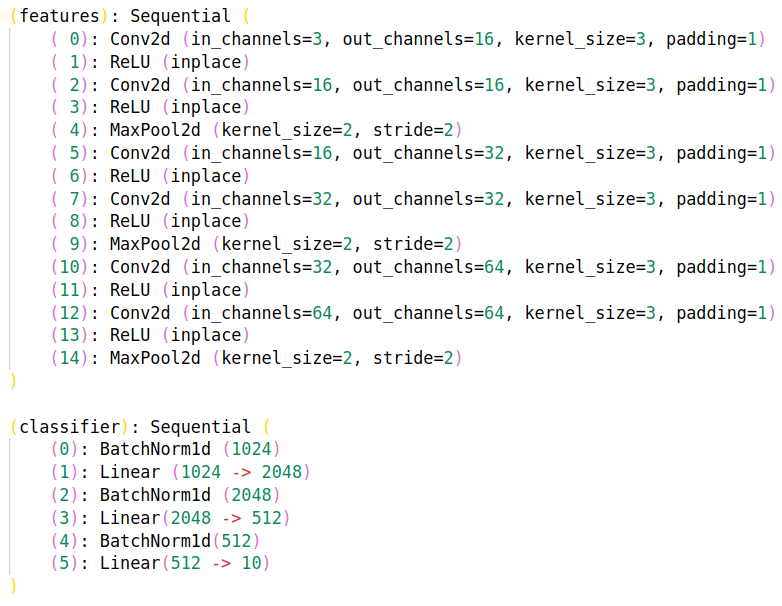
\includegraphics[width=\textwidth]{week4-cnn-architecture.png}
\caption{Convolutional Neural Network Architecture}
\end{figure}

\subsubsection{Result}
With batch\_size of 100, number of epochs of 100, learning\_rate of 1e-2; we have the train accuracy of 100\% (50000 / 50000) and the test error of 28.37\% (2837 / 10000).

All my work and trained model could be found \href{https://gitlab.com/tlvu2697/image-classification-cifar10}{here}.